\documentclass[11pt,a4paper]{article}

\usepackage{fontspec}
\usepackage{polyglossia}
\setdefaultlanguage[script=Latin]{serbian}
\setotherlanguage{english}

\usepackage[margin=2.5cm]{geometry}
\usepackage{amsmath,amssymb}
\usepackage{booktabs,tabularx,array}
\usepackage{graphicx}
\usepackage{xcolor}
\usepackage{tikz}
\usetikzlibrary{arrows.meta,positioning,fit,calc}
\usepackage{listings}
\usepackage{caption}
\usepackage{enumitem}
\usepackage{microtype}
\usepackage[hidelinks]{hyperref}
\usepackage{float}

\lstset{
  basicstyle=\ttfamily\small,
  keywordstyle=\color{blue!60!black}\bfseries,
  commentstyle=\color{gray},
  stringstyle=\color{red!50!black},
  frame=leftline, framesep=3mm, xleftmargin=4mm,
  breaklines=true, columns=fullflexible, keepspaces=true,
  showstringspaces=false, tabsize=4,
  aboveskip=0.6em, belowskip=0.6em
}

\newcommand{\code}[1]{\texttt{\detokenize{#1}}}
\newcommand{\eng}[1]{(eng.~\textit{#1})}
\newcommand{\vect}[1]{\mathbf{#1}}

\setlength{\parindent}{0pt}
\setlength{\parskip}{0.6em}
\setlength{\emergencystretch}{3em}

\title{\textbf{dumbgrad}
  \\[0.3em]\large Dokumentacija softverskog alata za automatsko računanje
  gradijenata,\\ feedforward i rekurentne neuronske mreže}
\author{Ognjen Čavić}
\date{}

\begin{document}
\maketitle
\tableofcontents
\newpage

\section{Uvod}

\textit{dumbgrad} je softverski alat napisan u \textit{Python}-u za izgradnju i
obuku neuronskih mreža. Nastao je po uzoru na \textit{micrograd}~\cite{micrograd},
jezgro je izgradnja računskog grafa nad skalarnim vrednostima sa propagacijom
unazad, a iznad njega su neuroni, slojevi, \textit{LSTM} slojevi, funkcije gubitka,
regularizacija, optimizacija pomoću \textit{ADAM} algoritma i paralelno obučavanje
koje simulira federalno učenje.

\subsection{Struktura projekta}

\begin{center}
\begin{table}[h]
\begin{tabularx}{\textwidth}{>{\ttfamily}l X}
\toprule
\textrm{\textbf{Datoteka}} & \textbf{Sadržaj} \\
\midrule
dumbgrad/engine.py & klasa \code{Value}: izgradnja računskog grafa,
                     topološko sortiranje, ponovno izračunavanje i
                     propagacija gradijenta unazad \\
dumbgrad/graph.py  & iscrtavanje računskog grafa pomoću \textit{graphviz}-a \\
dumbgrad/utils.py  & pomoćne funkcije za transformaciju podataka \\
dumbgrad/nn.py     & funkcije gubitka, optimizator, regularizacija,
                       \code{Neuron}, \code{Layer}, \code{LSTM}, \code{Network} \\
examples/          & primeri upotrebe \\
tests/             & testovi ispravnosti pojedinačnih funkcionalnosti\\
\bottomrule
\end{tabularx}
\caption{Struktura projekta}
\end{table}
\end{center}

\subsection{Pokretanje}

Jezgro biblioteke (\code{engine}, \code{nn}, \code{utils}) koristi samo
standardnu biblioteku \textit{Python}-a, verzije 3.10 ili novije.
Izuzetak je modul \code{graph}, koji koristi \textit{graphviz}~\cite{graphviz}
za iscrtavanje računskih grafova. Primeri i testovi koriste dodatne pakete:
\begin{itemize}
  \item \textit{scikit-learn}~\cite{scikit-learn} ---
        skupove podataka i raspodelu na trening i test skupove u primerima
  \item \textit{requests}~\cite{requests} ---
        preuzimanje podataka sa udaljenih servera pomoću \textit{http} zahteva
  \item \textit{tkinter}~\cite{tkinter} ---
        kreiranje grafičkog interfejsa
  \item \textit{numpy}~\cite{numpy}
        --- referentne implementacije funkcija pomoću kojih
        se testira ispravnost funkcionalnosti \textit{dumbgrad} alata
\end{itemize}
Primeri i testovi se pokreću iz korenskog direktorijuma:

\begin{lstlisting}[language=bash]
pip install -r requirements.txt
python3 -m examples.iris        # jedan primer
python3 -m pytest tests         # svi testovi
\end{lstlisting}

Da bi izvršavanje testova i primera bilo uspešno, \textit{graphviz} i
\textit{tkinter} softverski paketi moraju biti instalirani na nivou celog
sistema, nije dovoljno da budu samo u virtuelnom okruženju. \textit{tkinter}
je deo standardne \textit{Windows} instalacije \textit{Python}-a, dok je
\textit{graphviz} neophodno skinuti posebno. Na \textit{Linux} sistemima je
oba paketa potrebno preuzeti pomoću menadžera paketa odgovarajuće distribucije.

\subsection{Oznake}

\begin{table}[h]
\centering
\begin{tabular}{cl}
\toprule
\textbf{Oznaka} & \textbf{Značenje} \\
\midrule
$x_i$, $\vect{x}$ & ulaz neurona, odnosno vektor ulaza \\
$w_i$, $b$ & težine i pomeraj \eng{bias} \\
$z$ & linearna kombinacija $b + \sum_i w_i x_i$ \\
$\varphi$ & aktivaciona funkcija \\
$\sigma$ & sigmoidna funkcija $\sigma(z) = 1/(1+e^{-z})$ \\
$y$, $\hat{y}$ & očekivani i predviđeni izlaz \\
$L$ & funkcija gubitka \\
$\vect{c}_t$ & dugoročna memorija ćelije LSTM u trenutku t \\
$\vect{h}_t$ & kratkoročna memorija ćelije LSTM u trenutku t \\
$\odot$ & množenje po elementima \\
$[\vect{a}, \vect{b}]$ & nadovezivanje vektora \\
$\theta$, $g$ & parametar i njegov gradijent $\partial L / \partial \theta$ \\
$\eta$ & stopa učenja \eng{learning rate} \\
\bottomrule
\end{tabular}
\caption{Oznake}
\end{table}

\section{Modul \texttt{engine}}
\label{sec:engine}

\subsection{Osnovni pojmovi}

\paragraph{Računski graf.} Svaki izraz se može predstaviti kao usmeren
aciklični graf čiji su čvorovi skalarne vrednosti. Vrednosti koje nisu nastale
nekom operacijom, kao što su ulazi i parametri, su listovi grafa.
Svaka druga vrednost je rezultat operacije ($+$, $\times$, $\tanh$, \dots)
i pamti tu operaciju, kao i svoje operande, koji su deca te vrednosti.
Grane vode od operanada ka rezultatu, a koren grafa je konačni rezultat,
npr.\ gubitak. Vrednost svakog rezultata zavisi samo od vrednosti njegove dece,
pa se ceo izraz izračunava obilaskom čvorova u topološkom redosledu,
gde se svaki čvor se obrađuje nakon njegove dece.

\paragraph{Propagacija unazad.} Za obučavanje je potreban gradijent gubitka
$L$ po svakom parametru. Propagacija unazad \eng{backpropagation} ga računa
jednim prolazom kroz graf, u obrnutom topološkom redosledu, primenom
pravila izvoda složene funkcije. Ako čvor $u$ ima roditelje $v_1, \dots, v_m$
(čvorove koji ga imaju kao dete), onda je
\begin{equation}
\frac{\partial L}{\partial u} = \sum_{i=1}^{m} \frac{\partial L}{\partial v_i}\,\frac{\partial v_i}{\partial u}.
\end{equation}
Svaki čvor zato treba da zna samo lokalni izvod svoje operacije
$\partial v / \partial u$; gradijent koji dolazi od roditelja množi lokalnim
izvodom i dodaje detetu.

\newpage

\subsection{Klasa \texttt{Value}}

\code{Value} je čvor računskog grafa. Konstruktor prima sledeće argumente:

\begin{table}[h]
\centering
\begin{tabularx}{\textwidth}{>{\ttfamily}l X}
\toprule
\textrm{\textbf{Polje}} & \textbf{Značenje} \\
\midrule
data & skalarna vrednost čvora \\
grad & gradijent $\partial y / \partial \text{data}$, gde je $y$ koren grafa, popunjava ga \code{backprop} \\
children & lista dece čvorova \\
  op & naziv operacije pod navodnicima (\code{'+'}, \code{'tanh'}, \dots), ili
       \code{None} \\
label & opcioni naziv, koristi se pri iscrtavanju grafa \\
\bottomrule
\end{tabularx}
\caption{Argumenti konstruktora klase \code{Value}}
\end{table}

Polja ove klase su definisana pomoću \code{__slots__}~\cite{slots} direktive,
čime se štedi memorija i ubrzava pristup.

\subsubsection{Operacije}

Operatori osnovnih aritmetičkih operacija su preklopljeni, pa se izrazi pišu
kao i kod običnih brojeva. Ako je jedan operand instanca klase \code{Value},
svi ostali operandi se automatski pretvaraju u objekte ove klase. Svaka
operacija pravi novi čvor, pamti decu i operaciju kojom je taj čvor nastao.
Tabela~\ref{tab:ops} sadrži primere, rezultate i računanje izvoda za operande
tog izraza.

\begin{table}[h]
\centering
\begin{tabular}{l l l l}
\toprule
\textbf{Upotreba} & \textbf{Vrednost $v$} & $\partial v/\partial a$ & $\partial v/\partial b$ \\
\midrule
\code{a + b} & $a+b$ & $1$ & $1$ \\
\code{a - b} & $a-b$ & $1$ & $-1$ \\
\code{a * b} & $ab$ & $b$ & $a$ \\
\code{a ** b} & $a^b$ & $b\,a^{b-1}$ & ne računa se \\
\code{a.tanh()} & $\tanh a$ & $1 - v^2$ & \\
\code{a.sigmoid()} & $\sigma(a)$ & $v(1-v)$ & \\
\code{a.relu()} & $\max(0,a)$ & $1$ ako je $a>0$, inače $0$ & \\
\code{a.leaky_relu()} & $a$ ako je $a\ge0$, inače $0.01a$ & $1$ ako je $a\ge0$, inače $0.01$ & \\
\code{a.exp()} & $e^a$ & $v$ & \\
\code{a.log()} & $\ln a$ & $1/a$ & \\
\code{a.abs()} & $|a|$ & $\operatorname{sgn}(a)$ & \\
\bottomrule
\end{tabular}
\caption{Operacije klase \code{Value} i njihovi lokalni izvodi}
\label{tab:ops}
\end{table}

Deljenje nije posebna operacija, $\frac{a}{b}$ se zapisuje kao \code{a * b ** -1}.
Kod operacije stepenovanja se izvod računa samo za osnovu, jer ne postoji potreba
za tim. Podržani su operatori poređenja $<$ i $>$, ali njihova upotreba ne pravi
nove čvorove, niti se njihova primena beleži, glavna svrha im je da funkcije poput
\code{min} i \code{argmax} budu primenjive nad \code{Value} objektima bez izmena.

Operacija koja nedostaje u tabeli~\ref{tab:ops} je linearna kombinacija dva
vektora i podržava dodavanje bias-a, implementirana je kao statička metoda
\code{Value.linear (weights, inputs, bias)}:
\begin{equation}
z = b + \sum_{i=1}^{n} w_i x_i,
\qquad
\frac{\partial z}{\partial w_i} = x_i,\quad
\frac{\partial z}{\partial x_i} = w_i,\quad
\frac{\partial z}{\partial b} = 1.
\label{eq:linear}
\end{equation}
Ova metoda kao rezultat vraća novi čvor, koji svoju decu čuva u vektoru
\code{[w_1, ..., w_n, x_1, ... x_n, b]}, pa je razdvajanje tokom propagiranja
unazad i ponovnog računanja jednostavno. Ukoliko su ulazni vektori različitih
veličina, ova metoda će prijaviti \vode{ValueError} izuzetak. Isti rezultat je
moguće dobiti pomoću operacija \code{+} i \code{*}, ali rezultuje većim grafom
računanja.

\subsubsection{\texttt{make\_topo()}}

Kreira topološki sortiranu listu svih čvorova koji su u srodstvu sa korenskim.
To podrazumeva njegovu decu, decu njihove dece, itd. To znači da je svaki čvor
dodat u topologiju nakon njegove dece.

Ova funkcija je implementirana kao iterativni obilazak u dubinu, jer \textit{Python}
ograničava dubinu rekurzije, što je problematično u slučaju velikih grafova.
Druga prednost ovog pristupa je redosled čvorova, svaki čvor će imati svu svoju
decu u topologiji pre njega, što se koristi kod obuke \textit{LSTM}-ova
nad sekvencama promenljive dužine.

\subsubsection{\texttt{backprop(topo)}}

Računa gradijente za svaki čvor u topologiji. Gradijent korenskog čvora,
onog nad kojim se metoda poziva, će biti 1 ($\frac{\partial y}{\partial y}=1$),
dok se za sve ostale čvorove određuje po formulama iz tabele~\ref{tab:ops} i
jednačine~\ref{eq:linear} pomnožen sa gradijenom roditelja. Budući da svaki
čvor može imati više od jednog roditelja, gradijenti se akumuliraju u tom čvoru.
To znači da se kasnije gradijenti moraju vratiti na nulu kako ne bi došlo do
greške.

\subsubsection{\texttt{recompute(topo, null\_grads=True)}}

Ponovo izračunava vrednost svakog čvora u topologiji, iz vrednosti njegove
dece, koristeći istu operaciju koja je čvor napravila.
Pored toga, opcija \code{null_grads} omogućuje usputno resetovanje gradijenata
svih posećenih čvorova na nulu.

Glavni princip rada celog alata se oslanja na upotrebu ove metode u kombinaciji
sa \code{backprop}. Operacije za obuku modela se pozivaju samo jednom, čime se
kreira računski graf, zatim se samo menjaju vrednosti ulaza za svaki uzorak u
skupu podataka i pozivaju operacije ponovnog računanja vrednosti i gradijenata.

\subsubsection{Primer upotrebe}

\begin{lstlisting}
from dumbgrad.engine import Value

x1, x2 = Value(1.0, label='x1'), Value(-2.0, label='x2')
w1, w2 = Value(0.5, label='w1'), Value(0.25, label='w2')
b = Value(0.1, label='b')

y = Value.linear([w1, w2], [x1, x2], b).tanh()   # y = tanh(b + w1 x1 + w2 x2)
topo = y.make_topo()     # [w1, w2, x1, x2, b, z, y]
y.backprop(topo)         # w1.grad = (1 - y^2) * x1, ...

x1.data = 3.0            # novi ulaz, isti graf
y.recompute(topo)        # y.data je sada tanh(0.1 + 1.5 - 0.5)
y.backprop(topo)
\end{lstlisting}

\newpage

\section{Modul \texttt{graph}}
\label{sec:graph}

Modul sadrži dve funkcije, preuzete su iz \textit{micrograd}
alata i adaptirane da rade sa \textit{dumbgrad} softverskim alatom:

\begin{itemize}[nosep]
  \item \code{trace(root)} --- poziva operaciju kreiranja topologije i pretvara
        je u skup\eng{set} torki\eng{tuple} svakog čvora sa svakim njegovim
        detetom.
\item \code{draw_dot(root)} --- vraća \code{graphviz.Digraph} u kom je svaki čvor
pravougaonik sa oznakom, vrednošću i gradijentom, a svaka operacija poseban
čvor između dece i rezultata.
\end{itemize}

Slika~\ref{fig:graph} sadrži rezultat poziva funkcije \code{draw_dot}, koji je sačuvan pomoću
\code{render} metode u datoteku. Sadržaj slike je računski graf izraza:
\begin{equation}
y = \tanh(x_1 \cdot w_1 + x_2 \cdot w_2 + b)
\end{equation}
Koji je predstavljen u kodu u ranijem primeru.
\begin{figure}[h]
\centering
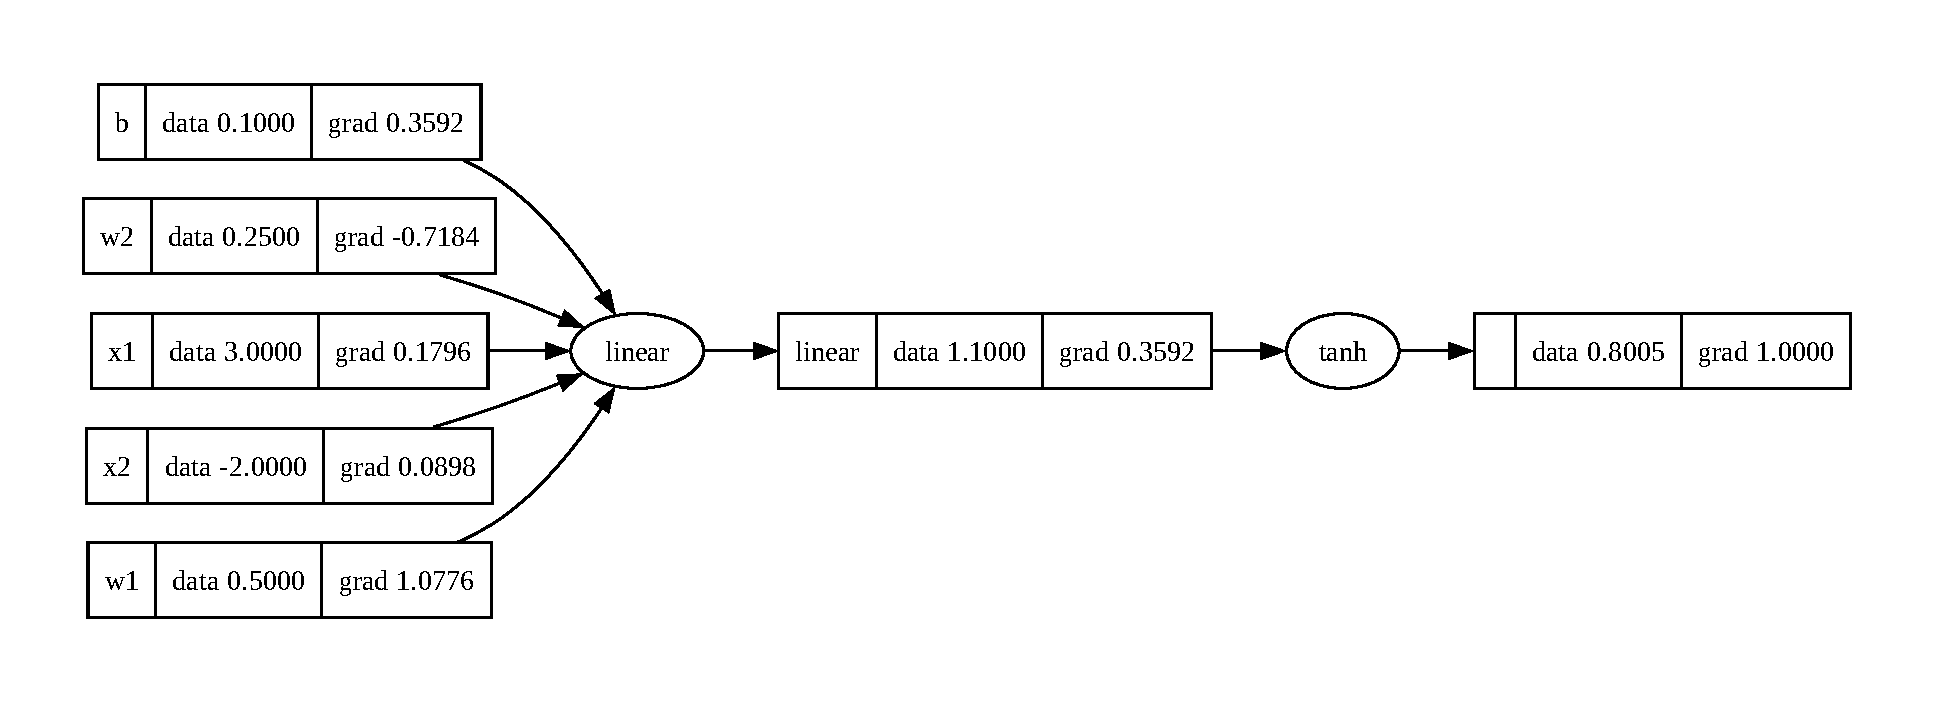
\includegraphics[width=0.85\textwidth]{fig/graph_neuron}
\caption{Primer prikaza računskog grafa}
\label{fig:graph}
\end{figure}
\vspace{-0.5cm}

\section{Modul \texttt{utils}}
\label{sec:utils}

Funkcije ovog modula se mogu podeliti u tri grupe:
\begin{itemize}
  \item Operacije nad listama --- izvlačenje osnovnih informacije iz jednog niza
  \item Operacije nad \code{Value} objektima --- prečice za operacije koje se
        često koriste
  \item Priprema podataka --- transformacije podataka tako da budu pogodni za
        prosleđivanje modelu
\end{itemize}

\subsection{Operacije nad listama}

Skup operacija pomoću kojih se izvlače osnovne informacije iz jednog niza. Rade
i sa običnim brojevima i sa \code{Value} objektima:

\begin{table}[H]
\begin{tabularx}{\textwidth}{>{\ttfamily}l X}
\toprule
\textrm{\textbf{Datoteka}} & \textbf{Sadržaj} \\
\midrule
  argmax & vraća indeks najvećeg elementa u nizu \\
  flatten & kreira novu listu gde su svi elementi poravnati u jednu dimenziju \\
  flat\_iter & iteriranje kroz niz kao da je jednodimenzionalan \\
  unique & prebrojavanje jedinstvenih elemenata \\
\bottomrule
\end{tabularx}
\caption{Funkcije operacija nad listama}
\end{table}

\subsection{Operacije nad \textttt{Value} objektima}

\subsubsection{\textttt{value\_sum (arr)}}

Sumira niz \code{Value} objekata. Moguće je i koristiti postojeću \code{sum}
funckiju u standardnoj biblioteci, ali ona inicijalizuje akumulator na nulu,
što će kreirati dodatni čvor. To znači da je graf računanja veći nego što je
potrebno, što usporava operacije nad grafom bez ikakvog dobitka.

\subsubsection{\texttt{update\_placeholders (placeholders, new\_values)}}

Ažuriranje pojedinačnih vrednosti već izgrađenog računskog grafa. Prvi argument
je lista čvorova čije vrednosti treba ažurirati, drugi argument su nove
vrednosti, ali kao obični brojevi, ne kao \code{Value} objekti. Ova funkcija
podržava i više dimenzionalne ulaze, jer se interno liste poravnaju. Ukoliko
je broj elemenata prosleđenih listi različit, greška neće biti prijavljena,
ali može dovesti do netačnih rezultata.

\subsection{Priprema podataka}
\subsubsection{\texttt{normalize(x, per\_column=False)}}

Skalira vrednosti na interval $[0, 1]$ min-maks normalizacijom:
\begin{equation}
x' = \frac{x - x_{\min}}{x_{\max} - x_{\min}}.
\label{eq:norm}
\end{equation}
Sa \code{per_column=False} minimum i maksimum se računaju nad celim skupom
(pogodno kada sve kolone imaju istu jedinicu, npr.\ pikseli slike), a sa
\code{per_column=True} posebno za svaku kolonu (pogodno kada kolone imaju
različite redove veličine, npr.\ dimenzije cveta, gde je jedna kolona većeg
opsega od druge).

Funkcija vraća novu listu i ne menja argument, pa se mora pisati
\code{x = normalize(x)}. Novi ulazi pri upotrebi modela (npr.\ u grafičkom
interfejsu) moraju biti skalirani na isti način kao trening skup.

\subsubsection{\texttt{to\_categorical(y, num\_classes=None)}} pretvara listu
celobrojnih indeksa klasa u \textit{one-hot} vektore. Broj klasa je
podrazumevano $\max(y) + 1$; ako se zada \code{num_classes}, vektori su te
dužine (manji broj od potrebnog izaziva \code{ValueError}). Zadavanje broja
klasa je neophodno kada se kodira samo deo podataka, u kome se najveća klasa
možda ne pojavljuje.
\begin{lstlisting}
>>> to_categorical([4, 2, 0])
[[0, 0, 0, 0, 1], [0, 0, 1, 0, 0], [1, 0, 0, 0, 0]]
>>> to_categorical([2, 0])
[[0, 0, 1], [1, 0, 0]]
>>> to_categorical([2, 0], num_classes=5)
[[0, 0, 1, 0, 0], [1, 0, 0, 0, 0]]
\end{lstlisting}

\subsubsection{\texttt{from\_categorical(y)}}
Obrnuta operacija od \code{to_categorical}, na ulazu se očekuje niz \textit{one-hot}
ulaza, gde se nad svakim poziva funkcija \code{argmax}.

\begin{lstlisting}
>>> from_categorical([[0, 0, 0, 0, 1], [0, 0, 1, 0, 0], [1, 0, 0, 0, 0]])
[4, 2, 0]
\end{lstlisting}

\subsubsection{\texttt{create\_mapping(arr, sort=True, per\_character=False)}}

Pravi rečnik koji svakoj jedinstvenoj vrednosti (klasi) dodeljuje indeks.
Vrednosti mogu biti brojevi, reči ili znakovi. Sa \code{sort=True} indeksi prate
sortiran redosled, a sa \code{sort=False} redosled pojavljivanja.
Sa \code{per_character=True}, za listu stringova klase su pojedinačni znakovi,
a ne celi stringovi.

\begin{lstlisting}
>>> create_mapping("dcba")
{'a': 0, 'b': 1, 'c': 2, 'd': 3}
>>> create_mapping("dcba", sort=False)
{'d': 0, 'c': 1, 'b': 2, 'a': 3}
>>> create_mapping(["ab", "ba"])
{'ab': 0, 'ba': 1}
>>> create_mapping(["ab", "ba"], per_character=True)
{'a': 0, 'b': 1}
\end{lstlisting}

\subsubsection{\texttt{encode\_labels(arr, per\_character=False, mapping=None)}}

Kodira proizvoljne oznake u \textit{one-hot} vektore: preslika ih u indekse
pomoću \code{mapping} (ako mapiranje nije dato, pravi ga \code{create_mapping}
iz dostavljenih podataka) i pozove \code{to_categorical} sa brojem klasa jednakim
veličini mapiranja. Sa \code{per_character=True} vraća po jednu matricu za
svaki string, sa jednim vektorom po znaku; to je oblik koji očekuje
obuka \textit{LSTM} mreže.

Kod jezičkih modela mapiranje treba praviti jednom, iz fiksnog skupa znakova,
i isto mapiranje koristiti i pri obučavanju i pri upotrebi modela. Kada bi se
mapiranje pravilo iz podataka, znak koji se u nekom delu podataka ne pojavljuje
bi pomerio indekse svih znakova posle njega.

\begin{lstlisting}
CHARACTERS = sorted(set("abcčćdđefghijklmnoprsštuvzž .,!?#"))
mapping = create_mapping(CHARACTERS)
encoded = encode_labels(["kako si", "dobro"], per_character=True, mapping=mapping)
\end{lstlisting}

\subsubsection{\texttt{make\_batches(inputs, outputs, batch\_size)}}

Deli skup podataka na šarže \eng{batch} od \code{batch_size} uzoraka. Ulazi i
očekivani izlazi se dele u dve odvojene matrice, tako da svaka šarža ulaza ima
odgovarajuću šaržu izlaza. Ako broj uzoraka nije deljiv veličinom šarže,
nepotpuna šarža se odbacuje.

\begin{lstlisting}
>>> make_batches([1, 2, 3, 4, 5], ['a', 'b', 'c', 'd', 'e'], 2)
([[1, 2], [3, 4]], [['a', 'b'], ['c', 'd']])
\end{lstlisting}

\subsubsection{\texttt{array\_split(array, n)}}

Pokušava da podeli listu \code{array} na \code{n} delova jednake dužine. Ako
dužina liste $l$ nije deljiva sa $n$, $\frac{l}{n}=k$ sa ostatkom $m$, tada će
prvih $m$ nizova imati $k+1$ elemenata. Za razliku od \code{make_batches}, koja
raspodeljuje niz na pod-nizove fiksne veličine i odbacuje ostatak, ova funkcija
raspodeljuje niz na fiksan broj pod-nizova i ne odbacuje nijedan element.
Koristi se za raspodelu podataka po procesima tokom obuke.

\begin{lstlisting}
>>> array_split([10, 9, 8, 7, 6, 5, 4, 3, 2, 1], 4)
[[10, 9, 8], [7, 6, 5], [4, 3], [2, 1]]
>>> array_split([1, 2], 3)
[[1], [2], []]
\end{lstlisting}

\section{Modul \texttt{nn}: neuronske mreže}
\label{sec:nn}

Modul \code{nn} gradi neuronske mreže od \code{Value} čvorova. Sve klase
koriste isti princip: poziv sloja ili mreže nad listom \code{Value} objekata
vraća nove \code{Value} objekte, odnosno proširuje računski graf, a
gradijenti se dobijaju pozivom \code{backprop} nad gubitkom.

\subsection{Klasa \texttt{Parameter}}

Klasa izvedena iz \code{Value}, predstavlja parametar koji se ažurira tokom
obuke (težina ili bias). Na roditeljsku klasu dodaje polja \code{m} i \code{v},
koja koristi \textit{ADAM} algoritam optimizacije.

\subsection{Klasa \texttt{Input}}

Nema interne parametre niti ikakvo računanje, jedina svrha ove klase je opisivanje
broja ulaza u model. Nakon potpune inicijalizacije modela ovaj sloj se uklanja.

\subsection{Klasa \texttt{Neuron}}

Neuron je najmanja gradivna jedinica neuronske mreže. Konstruktor prima
sledeće argumente:

\begin{table}[h]
\begin{tabularx}{\textwidth}{>{\ttfamily}l X}
\toprule
\textrm{\textbf{Polje}} & \textbf{Značenje} \\
\midrule
input\_count & broj ulaza neurona \\
  output\_count & broj neurona u sloju kojem neuron pripada \\
rng & objekat za generaciju nasumičnih brojeva po kojem se generišu parametri \\
activation & naziv aktivacione funkcije pod navodnicima \\
\bottomrule
\end{tabularx}
\caption{Argumenti konstruktora klase \code{Neuron}}
\end{table}

Neuron se inicijalizuje sa \code{input_count} težina pomoću lambda izraza koji se
dobija sa \code{make_weight_lambda(limit, rng)}. Svaki poziv tog izraza pravi
novi \code{Parameter} sa vrednošću iz uniformne raspodele
$\mathcal{U}(-\text{limit}, \text{limit})$, gde se granica računa po
Ksavijerovoj formuli~\cite{xavier}
\begin{equation}
\text{limit} = \sqrt{\frac{6}{\text{input\_count} + \text{output\_count}}}.
\label{eq:xavier}
\end{equation}

Ako je \code{rng} napravljen sa \code{random.Random(seed)}, gde je \code{seed}
seme generisanja težina, tada je moguće ostvariti iste početne težine između
pokretanja, čime se omogućuje ponovljivost obuke.

Poziv kreiranog objekta neurona nad listom ulaza \code{neuron(x)}, računa
linearnu kombinaciju ulaza i na nju primenjuje aktivacionu funkciju:
\begin{equation}
y = \varphi\!\left(b + \sum_{i=1}^{n} w_i x_i\right).
\label{eq:neuron}
\end{equation}

Nelinearna aktivacija je ono što mreži omogućava da uči nelinearne zavisnosti,
podržane su sledeće aktivacione funkcije:

\begin{table}[H]
\centering
\begin{tabular}{l l l l}
\toprule
\textbf{\texttt{activation}} & $\varphi(z)$ & $\varphi'(z)$ & \textbf{Opseg} \\
\midrule
\code{"tanh"} & $\tanh z$ & $1-\tanh^2 z$ & $(-1, 1)$ \\
\code{"sigmoid"} & $\sigma(z)$ & $\sigma(z)(1-\sigma(z))$ & $(0, 1)$ \\
\code{"relu"} & $\max(0, z)$ & $[z > 0]$ & $[0, \infty)$ \\
\code{"leaky_relu"} & $\max(0.01z, z)$ & $1$ ili $0.01$ & $\mathbb{R}$ \\
\code{"softmax"} & $e^z$ (normalizuje sloj) & & $(0, 1)$ \\
\bottomrule
\end{tabular}
\caption{Podržane aktivacione funkcije}
\end{table}

Kod \code{"softmax"} neuron računa samo $e^z$; normalizaciju na zbir $1$
obavlja sloj. Nepoznat naziv aktivacije izaziva \code{ValueError}.

Parametri neurona, a kasnije i čitave mreže, dobijaju se metodom
\code{parameters()}, koja vraća listu svih parametara. Lista je plitka kopija
\eng{shallow copy}, što znači da promena vrednosti parametra preko te liste
menja i sam neuron, što se koristi tokom obuke.

\subsection{Klasa \texttt{Layer}}
\label{sec:layer}

Sloj\eng{layer} je potpuno povezan sloj neurona. Da bi se sloj kreirao potrebni
su argumenti:

\begin{table}[h]
\begin{tabularx}{\textwidth}{>{\ttfamily}l X}
\toprule
\textrm{\textbf{Polje}} & \textbf{Značenje} \\
\midrule
size & broj neurona u sloju \\
activation & naziv aktivacione funkcije za sve neurone u sloju pod navodnicima \\
\bottomrule
\end{tabularx}
\caption{Argumenti konstruktora klase \code{Layer}}
\end{table}

Konstruktor samo pamti broj neurona i aktivaciju, a neuroni se prave kad se
pozove \code{build(input_count, rng=None)} kada je poznat broj ulaza sloja.
Svaki neuron dobija \code{input_count} ulaza, a \code{size} se prosleđuje kao
\code{output_count} za inicijalizaciju.

Pozivom sloja nad listom ulaza, ista lista se prosleđuje svakom neuronu, a
rezultat je lista izlaza svih neurona, dužine \code{size}. Pošto svaki neuron
vidi sve ulaze, sloj je potpuno povezan. Za ceo sloj odjednom to se može
zapisati kao:
\begin{equation}
\vect{y} = \varphi(W\vect{x} + \vect{b}),
\label{eq:layer}
\end{equation}
Gde je $i$-ti red matrice $W$ lista težina $i$-tog neurona.

Kao i kod neurona, parametri sloja se dobijaju metodom \code{parameters()}, a
samo težine, bez pomeraja, metodom \code{weights()}, koju koristi
regularizacija. Obe metode spajaju liste svih neurona u jednu, i takođe
vraćaju reference na iste \code{Parameter} objekte.

\subsubsection{Softmax}

Ako je aktivaciona funkcija postavljena na \code{softmax}, pri pozivu svaki
neuron računa $e^{z_i}$, zatim se ti izlazi sabiraju i svaki se posebno deli
tim zbirom:
\begin{equation}
\hat{y}_i = \frac{e^{z_i}}{\sum_j e^{z_j}}.
\label{eq:softmax}
\end{equation}
Tako su svi izlazi pozitivni i zbir im je $1$, pa predstavljaju raspodelu
verovatnoća po klasama.

\subsection{Klasa \texttt{LSTM}}

\textit{LSTM}~\cite{lstm} je rekurentni sloj, koji obrađuje sekvencu element
po element i između koraka pamti stanje: dugoročnu memoriju $\vect{c}_t$ i
kratkoročnu memoriju $\vect{h}_t$, koja je ujedno i izlaz sloja. Da bi se sloj
kreirao potreban je argument:

\begin{table}[h]
\begin{tabularx}{\textwidth}{>{\ttfamily}l X}
\toprule
\textrm{\textbf{Polje}} & \textbf{Značenje} \\
\midrule
size & dužina memorija $\vect{c}_t$ i $\vect{h}_t$, odnosno broj izlaza sloja \\
\bottomrule
\end{tabularx}
\caption{Argument konstruktora klase \code{LSTM}}
\end{table}

Kao i kod sloja, konstruktor samo pamti veličinu, a težine se prave pozivom
\code{build(input_count, rng=None)}. Za svaku od četiri kapije pravi se
matrica težina za kratkoročnu memoriju, matrica težina za ulaz i bias, a
težine se inicijalizuju po~\eqref{eq:xavier}. Obe memorije se postavljaju na
nulu.

Jedan poziv sloja nad listom ulaza je jedan korak sekvence. Prvo se računaju
četiri kapije, gde je svaki element kapije linearna kombinacija nadovezane
kratkoročne memorije i ulaza, na koju se primenjuje aktivaciona funkcija:
\begin{align}
\vect{f}_t &= \sigma\big(W_f [\vect{h}_{t-1}, \vect{x}_t] + \vect{b}_f\big), &
\vect{i}_t &= \sigma\big(W_i [\vect{h}_{t-1}, \vect{x}_t] + \vect{b}_i\big), \label{eq:lstm_kapije}\\
\vect{g}_t &= \tanh\big(W_c [\vect{h}_{t-1}, \vect{x}_t] + \vect{b}_c\big), &
\vect{o}_t &= \sigma\big(W_o [\vect{h}_{t-1}, \vect{x}_t] + \vect{b}_o\big). \notag
\end{align}
Kapija zaboravljanja $\vect{f}_t$ određuje koliki deo dugoročne memorije
ostaje, ulazna kapija $\vect{i}_t$ koliki deo kandidata $\vect{g}_t$ se
upisuje, a izlazna kapija $\vect{o}_t$ koliki deo memorije postaje izlaz.
Zatim se računaju nove memorije:
\begin{align}
\vect{c}_t &= \vect{f}_t \odot \vect{c}_{t-1} + \vect{i}_t \odot \vect{g}_t, \label{eq:lstm_c}\\
\vect{h}_t &= \vect{o}_t \odot \tanh(\vect{c}_t). \label{eq:lstm_h}
\end{align}

Memorije se čuvaju u objektu, pa svaki poziv nastavlja od prethodnog. Zato se
na prvom elementu svake sekvence sloj poziva sa \code{reset=True}, čime se
memorije vraćaju na nulu. U suprotnom bi nova sekvenca nastavila iz memorije
prethodne. Metode \code{parameters()} i \code{weights()} rade isto kao kod
sloja.

\subsubsection{Odvijanje kroz vreme}

Ako se pozivi za jednu sekvencu nacrtaju jedan pored drugog, dobija se
odvijena \eng{unrolled} mreža, prikazana na slici~\ref{fig:lstm_unroll}. Slojevi
ispred i iza \textit{LSTM}-a se primenjuju na svaki korak posebno, sa istim
težinama, i ne znaju ništa o prethodnim koracima. Jedino \textit{LSTM} prenosi
stanje iz koraka u korak.

\begin{figure}[H]
\centering
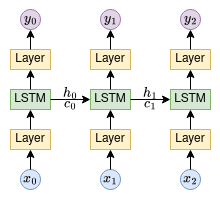
\includegraphics[width=0.35\textwidth]{fig/lstm_unroll.png}
\caption{Odvijanje mreže sa \textit{LSTM}}
\label{fig:lstm_unroll}
\end{figure}

Pošto se cela odvijena mreža gradi kao jedan računski graf, gubitak sekvence je
zbir gubitaka svih koraka, a propagacija unazad kroz vreme
\eng{backpropagation through time} je obična propagacija unazad kroz taj graf.
Isti \code{Parameter} objekti se koriste u svakom koraku, pa se njihovi
gradijenti sabiraju po svim koracima, isto kao kod čvora sa više roditelja.

\subsection{Funkcije gubitka}

Funkcija gubitka meri koliko se predviđanje $\hat{y}$ razlikuje od očekivanog
izlaza $y$, a obuka teži da je minimizuje. Obe funkcije primaju dve
dvodimenzionalne liste: prva sadrži očekivane izlaze, a druga predviđanja
modela za iste uzorke. Liste se poravnavaju pomoću \code{flat_iter}, a
rezultat je jedan \code{Value} čvor.

\subsubsection{\texttt{sum\_of\_squares(y, y\_pred)}}

Zbir kvadrata grešaka, pogodan za regresiju:
\begin{equation}
L = \sum_i (y_i - \hat{y}_i)^2,
\qquad
\frac{\partial L}{\partial \hat{y}_i} = -2(y_i - \hat{y}_i).
\label{eq:sos}
\end{equation}

\subsubsection{\texttt{cross\_entropy(y, y\_pred)}}

Unakrsna entropija \eng{cross-entropy}, pogodna za klasifikaciju. Ako je $y$
\textit{one-hot} vektor tačne klase, a $\hat{y}$ raspodela verovatnoća koju
daje mreža, onda je:
\begin{equation}
L = -\sum_i y_i \ln \hat{y}_i,
\label{eq:ce}
\end{equation}
Odnosno negativan logaritam verovatnoće koju je mreža dodelila tačnoj klasi.
Gubitak je nula kada je ta verovatnoća $1$, a raste neograničeno kada teži
nuli, pa je mreža strogo kažnjena za samouvereno pogrešna predviđanja. Zato
se koristi zajedno sa \textit{softmax} izlazom~\eqref{eq:softmax}.

\subsection{Regularizacija}

Regularizacija dodaje gubitku kaznu za velike težine, čime se smanjuje
preterano prilagođavanje trening skupu \eng{overfitting}. Ukupan gubitak koji
se minimizuje je
\begin{equation}
L_\text{ukupno} = L + R(\vect{w}),
\label{eq:reg}
\end{equation}
gde je $R$ kazna, a $\vect{w}$ sve težine mreže, bez biasa.

Sve klase regularizacije su izvedene iz bazne klase \code{Regularization},
koja čuva koeficijent $\alpha$ (podrazumevano $0.01$). Poziv objekta nad
listom težina vraća kaznu kao \code{Value} čvor:

\begin{table}[h]
\centering
\begin{tabular}{l l}
\toprule
\textbf{Klasa} & \textbf{Kazna $R$} \\
\midrule
\code{L1Regularization} & $\alpha \sum_i |w_i|$ \\
\code{L2Regularization} & $\alpha \sum_i w_i^2$ \\
\code{NoRegularization} & $0$ \\
\bottomrule
\end{tabular}
\caption{Podržane klase regularizacije}
\end{table}

L2 kazna smanjuje sve težine srazmerno njihovoj veličini, dok L1 kazna gura
nebitne težine tačno na nulu, pa model koristi manji broj težina. Ako
regularizacija nije zadata, koristi se \code{NoRegularization}.

\subsection{Algoritam optimizacije --- klasa \texttt{Optimizer} (ADAM)}

Klasa \code{Optimizer} implementira \textit{ADAM} algoritam optimizacije.
Konstruktor prima sledeće argumente:

\begin{table}[h]
\begin{tabular}{>{\ttfamily}l c l l}
\toprule
\textrm{\textbf{Argument}} & \textbf{Oznaka} & \textbf{Podrazumevano} & \textbf{Značenje} \\
\midrule
omega1 & $\omega_1$ & $0.9$ & koliko se pamte prethodni gradijenti \\
omega2 & $\omega_2$ & $0.99$ & koliko se pamte prethodni kvadrati gradijenata \\
lr & $\eta$ & $0.001$ & stopa učenja \\
eps & $\varepsilon$ & $10^{-6}$ & sprečava deljenje nulom \\
\bottomrule
\end{tabular}
\caption{Argumenti konstruktora klase \code{Optimizer}}
\end{table}

Poziv \code{optimizer(p, t)} ažurira parametar \code{p} na osnovu njegovog
gradijenta $g$ (\code{p.grad}), gde je \code{t} redni broj koraka, počevši od
$1$. Parameter u poljima \code{m} i \code{v} čuva vrednosti koje se u svakom
koraku osvežavaju:
\begin{align}
m_t &= \omega_1 m_{t-1} + (1-\omega_1)\, g_t, &
v_t &= \omega_2 v_{t-1} + (1-\omega_2)\, g_t^2, \label{eq:adam1}\\
\hat{m}_t &= \frac{m_t}{1-\omega_1^t}, &
\hat{v}_t &= \frac{v_t}{1-\omega_2^t}, \label{eq:adam2}\\
\theta_t &= \theta_{t-1} - \eta\,\frac{\hat{m}_t}{\sqrt{\hat{v}_t} + \varepsilon}. \label{eq:adam3}
\end{align}
$m$ određuje smer koraka i ublažava šum pojedinačnih gradijenata, a $v$
procenjuje njihovu veličinu, pa svaki parametar dobija sopstvenu stopu učenja.
Pošto su $m$ i $v$ inicijalno jednaki nuli, u ranim koracima su premale, te
se koriste korigovane vrednosti $\hat{m}$ i $\hat{v}$.

\subsection{Klasa \texttt{Network}}
\label{sec:network}

Mreža povezuje slojeve u celinu i sadrži obuku, testiranje, čuvanje i
učitavanje modela. Konstruktor prima listu slojeva, čiji prvi element mora
biti \code{Input}, inače se baca \code{TypeError} izuzetak.
Slojevi se mogu kombinovati proizvoljno:

\begin{lstlisting}
n = Network([
    Input(5),
    Layer(10, activation="tanh"),
    LSTM(20),
    Layer(5, activation="softmax")
])
\end{lstlisting}

Pozivom mreže nad listom ulaza, ulaz se prosleđuje kroz sve slojeve redom, a
rezultat je izlaz poslednjeg sloja. Ulaz može biti lista brojeva ili lista
\code{Value} objekata. Kod rekurentne mreže jedan poziv je jedan korak
sekvence, a argument \code{reset} se prosleđuje samo \textit{LSTM} slojevima.
Kao i kod sloja, metode \code{parameters()} i \code{weights()} vraćaju
parametre, odnosno težine, svih slojeva.

\subsubsection{\texttt{build}}

Priprema mrežu za upotrebu. Prima sledeće argumente:

\begin{table}[h]
\begin{tabularx}{\textwidth}{>{\ttfamily}l X}
\toprule
\textrm{\textbf{Argument}} & \textbf{Značenje} \\
\midrule
seed & seme generatora nasumičnih brojeva, ako je zadato inicijalizacija
       težina je ponovljiva \\
loss & naziv funkcije gubitka, \code{"cross_entropy"} ili
       \code{"sum_of_squares"}, svaka druga vrednost izaziva \code{ValueError} \\
optimizer & objekat klase \code{Optimizer}, podrazumevano \code{Optimizer()} \\
regularization & objekat regularizacije podrazumevano \code{NoRegularization()} \\
\bottomrule
\end{tabularx}
\caption{Argumenti metode \code{build}}
\end{table}

Svaki sloj se gradi sa brojem ulaza jednakim veličini prethodnog sloja, a
\code{Input} sloj se nakon toga uklanja. Zato se \code{build} ne sme pozivati
dva puta nad istom mrežom.

\begin{lstlisting}
n.build(seed=0, loss="cross_entropy",
        optimizer=Optimizer(lr=0.01),
        regularization=L2Regularization())
\end{lstlisting}

\subsubsection{\texttt{train}}

Obučava mrežu. Prima sledeće argumente:

\begin{table}[h]
\begin{tabularx}{\textwidth}{>{\ttfamily}l X}
\toprule
\textrm{\textbf{Argument}} & \textbf{Značenje} \\
\midrule
inputs & ulazi skupa za obuku \\
outputs & očekivani izlazi, po jedan za svaki ulaz \\
batch\_size & broj uzoraka u šarži; koristi se samo kod \textit{feedforward}
              mreža, podrazumevano $1$ \\
epochs & broj epoha, podrazumevano $10$ \\
n\_workers & broj procesa koji paralelno obučavaju mrežu, podrazumevano $1$ \\
max\_time & najduže trajanje obuke u sekundama; podrazumevano bez
            ograničenja \\
\bottomrule
\end{tabularx}
\caption{Argumenti metode \code{train}}
\end{table}

Kod \textit{feedforward} mreže \code{inputs} i \code{outputs} su
dvodimenzionalne liste: lista uzoraka, gde je svaki uzorak lista brojeva. Na
primer, za funkciju logičkog ekskluzivnog ili \textit{XOR}:

\begin{lstlisting}
inputs  = [[0, 0], [1, 0], [0, 1], [1, 1]]
outputs = [[1, 0], [0, 1], [0, 1], [1, 0]]
# na izlazu se ocekuje:
#    [1, 0] za logicku 0
#    [0, 1] za logicka 1
\end{lstlisting}

Kod rekurentne mreže \code{inputs} i \code{outputs} su trodimenzionalni: lista
sekvenci, gde je svaka sekvenca lista uzoraka, a svaki uzorak lista brojeva.
Sekvence mogu biti različitih dužina, a \code{outputs[s][t]} je očekivani izlaz
za \code{inputs[s][t]}. Na primer, za predviđanje sledećeg znaka u rečima „ab“ i „bca“:

\begin{lstlisting}
# a = [1, 0, 0], b = [0, 1, 0], c = [0, 0, 1]
inputs  = [
  [[1, 0, 0]],              # "a"
  [[0, 1, 0], [0, 0, 1]]    # "bc"
]
outputs = [
  [[0, 1, 0]],              # "b"
  [[0, 0, 1], [1, 0, 0]]    # "ca"
]
\end{lstlisting}

\textit{Feedforward} mreža deli podatke u šarže od \code{batch_size}
uzoraka, dok se kod rekurentne mreže podaci ne dele, jer je svaka sekvenca već
grupa uzoraka. U oba slučaja ostatak obuke radi sa listom jedinica iste
strukture: šaržom uzoraka, odnosno sekvencom koraka.

Obuka je paralelizovana tako da simulira federalno učenje \textit{FedSGD}
metodom. Pravi se \code{n_workers} procesa, gde svaki dobija svoj deo
podataka. U svakoj epohi glavni proces šalje radnicima trenutne vrednosti
parametara, a svaki radnik računa gradijent svakog parametra nad celim svojim
delom podataka i šalje ga nazad. Glavni proces zatim usrednjava gradijente
svih radnika i primenjuje jedan korak optimizatora:
\begin{align}
\vect{g} = \frac{1}{N} \sum_{k=1}^{\text{n\_workers}} \vect{g}_k. &&
\theta = ADAM(\theta, g, t)
\label{eq:fedsgd}
\end{align}
Gde je $\vect{g}$ vektor uprosečenih gradijenata svih radnika, $N$ je broj uzoraka
nad kojim se model obučava, $\vect{g}_k$ je vektor gradijenata dobijenih od
radnika $k$.

\begin{figure}[h]
\centering
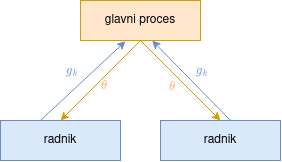
\includegraphics[width=0.45\textwidth]{fig/fedsgd.png}
\caption{Prikaz komunikacije između radnika i glavnog procesa}
\label{fig:fedsgd}
\end{figure}

Radnici su procesi, a ne niti, jer \textit{Python} ne dozvoljava paralelno
izvršavanje niti. Komuniciraju sa glavnim procesom kroz redove
(\code{multiprocessing.Queue}), šalju se samo brojevi, a ne \code{Parameter}
objekti. Ako odgovor radnika ne stigne pre isteka \code{max_time}, prijavljuje
se \code{queue.Empty} izuzetak, a radnici se gase zajedno sa glavnim procesom.
Broj radnika se smanjuje ako ima manje jedinica nego radnika, a više radnika
od broja jezgara procesora ne ubrzava obuku.

\subsubsection{\texttt{training\_worker}}

Radnik gradi računski graf samo jednom. Ulazi i očekivani izlazi grafa su
čvorovi čije se vrednosti dinamički menjaju: za svaku jedinicu radnik upiše
nove vrednosti u njih, pozove \code{recompute} i \code{backprop}, i sabere
gradijente parametara.

Problem je što graf napravljen za sekvencu jedne dužine ne odgovara sekvenci
druge dužine. Zato se graf gradi za najdužu sekvencu, a gubitak se gradi kao
zbir gubitaka svih koraka do tog trenutka. Ako je $L_k$ gubitak koraka $k$, a
$L_{1:k}$ gubitak prvih $k$ koraka:
\begin{equation}
L_{1:1} = L_1 + R(\vect{w}), \qquad L_{1:k} = L_{1:k-1} + L_k.
\label{eq:tekuci}
\end{equation}
Sekvenca dužine $k$ koristi gubitak $L_{1:k}$. Prethodni zbir je uvek prvi
operand, a \code{make_topo} obilazi decu redom, pa ceo podgraf od $L_{1:k-1}$
dolazi u topologiji pre bilo kog čvora koraka $k$. Zato je topologija od
$L_{1:k}$ tačno početni deo topologije celog grafa, i radnik za sekvencu
dužine $k$ poziva \code{recompute} i \code{backprop} samo nad tim delom.
Regularizacija se dodaje samo u $L_{1:1}$, pa je svaki zbir sadrži tačno jednom.

Kod \textit{feedforward} mreže isti postupak radi bez izmena: koraci su
uzorci šarže, a pošto su sve šarže iste dužine, uvek se koristi gubitak cele
šarže.

\subsubsection{\texttt{test}}

Vraća tačnost mreže, udeo predviđanja kod kojih je indeks najvećeg izlaza
jednak indeksu najvećeg očekivanog izlaza:
\begin{equation}
\text{tačnost} = \frac{1}{N}\sum_{j=1}^{N} \big[\operatorname{argmax} \hat{y}_j = \operatorname{argmax} y_j\big].
\label{eq:tacnost}
\end{equation}
Argumenti \code{inputs}, \code{outputs} i \code{n_workers} imaju isto značenje
kao kod \code{train}. Kod rekurentne mreže svaki korak sekvence je jedno
predviđanje, pa je $N$ ukupan broj koraka svih sekvenci. Uzorci mreže
\textit{feedforward} mreže se tretiraju kao sekvence dužine $1$, pa oba slučaja
obrađuje isti radnik.

Radnik za testiranje gradi graf za najdužu sekvencu i sva predviđanja vezuje
za jedan pomoćni čvor, čija topologija obuhvata ceo graf. Za svaku sekvencu
upiše nove ulaze, pozove \code{recompute} i uporedi predviđanja sa
očekivanim izlazima. U slučaju kraće sekvence, ponovno računanje će računati
i izlaze za kasnije korake, ali oni neće biti upoređivani.

\subsubsection{\texttt{save} i \texttt{load}}

Metoda \code{save(path)} upisuje mrežu u \textit{JSON} datoteku: parametre
optimizatora, regularizaciju, funkciju gubitka, opis slojeva i vrednosti svih
parametara redosledom \code{parameters()}. Statička metoda
\code{Network.load(path)} od opisa slojeva pravi istu mrežu, gradi je, i
nasumično inicijalizovane parametre zamenjuje sačuvanim vrednostima.

\begin{lstlisting}
{
    "optimizer": {"omega1": 0.9, "omega2": 0.99, "lr": 0.01, "eps": 1e-06},
    "regularization": {"type": "L2Regularization", "alpha": 0.01},
    "loss": "cross_entropy",
    "layers": [
        {"type": "Input", "size": 64},
        {"type": "Layer", "size": 30, "activation": "tanh"},
        {"type": "Layer", "size": 10, "activation": "softmax"}
    ],
    "parameters": [0.0213, -0.1879, ...]
}
\end{lstlisting}

Stanje optimizatora ($m$ i $v$) se ne čuva, pa je učitan model spreman za
predviđanje, a nastavak obuke počinje sa novim stanjem optimizatora.

\begin{lstlisting}
n.save("./examples/nets/digits.json")
m = Network.load("./examples/nets/digits.json")
m(x)        # isto predvidjanje kao n(x)
\end{lstlisting}

\section{Primeri}
\label{sec:primeri}

Svi primeri se nalaze u direktorijumu \code{examples/} i pokreću se iz
korenskog direktorijuma, npr.\ \code{python3 -m examples.iris}.

\subsection{Klasifikacija: \texttt{iris}, \texttt{breast\_cancer}, \texttt{mushroom}, \texttt{digits}}

Ovi primeri imaju istu strukturu i pokazuju osnovnu upotrebu alata: podaci se
učitavaju, normalizuju, klase se kodiraju \textit{one-hot}
vektorima, a mreža ima \textit{softmax} izlaz i obučava se
sa unakrsnom entropijom i L2 regularizacijom. Podaci se dele na
skup za obuku i test skup od 30\%, koji mreža ne vidi tokom obuke.

\begin{lstlisting}
dataset = load_iris()
x, y = dataset.data.tolist(), dataset.target.tolist()
x = normalize(x, per_column=True)
num_classes = len(unique(y))
y = to_categorical(y)
x_train, x_test, y_train, y_test = train_test_split(
    x, y, test_size=0.3, shuffle=True, random_state=0)

n = Network([
    Input(len(x[0])),
    Layer(30),
    Layer(num_classes, activation="softmax")
])
n.build(seed=0, loss="cross_entropy",
        regularization=L2Regularization(), optimizer=Optimizer(lr=0.01))
n.train(x_train, y_train, epochs=150, batch_size=50, n_workers=2)
n.test(x_test, y_test, n_workers=2)
\end{lstlisting}

Tabela~\ref{tab:results} prikazuje skupove podataka, mreže i tačnost na test
skupu.

\begin{table}[h]
\centering
\begin{tabular}{l r r r l r r}
\toprule
\textbf{Primer} & \textbf{Uzorci} & \textbf{Ulazi} & \textbf{Klase} &
\textbf{Skriveni slojevi} & \textbf{Epohe} & \textbf{Tačnost} \\
\midrule
\code{iris}          & 150  & 4   & 3  & 30     & 150 & 97.8\% \\
\code{breast_cancer} & 569  & 30  & 2  & 30, 30 & 15  & 78.4\% \\
\code{mushroom}      & 8416 & 117 & 2  & 30, 30 & 10  & 98.9\% \\
\code{digits}        & 1797 & 64  & 10 & 30, 30 & 20  & 89.3\% \\
\bottomrule
\end{tabular}
\caption{Skupovi podataka i rezultati klasifikacionih primera}
\label{tab:results}
\end{table}

\subsection{Crtanje cifara: \texttt{draw}}

Primer \code{draw} je grafički interfejs (\textit{tkinter}) u kom korisnik
crta cifru na mreži $8\times8$ polja, a model iz primera \code{digits} je
prepoznaje posle svakog klika. Graf mreže se pravi samo jednom, a svaki klik
menja vrednost jednog ulaza i poziva \code{recompute}, isto kao tokom obuke.

Polja imaju vrednosti $0$ i $1$, što odgovara normalizovanom skupu za obuku,
gde je $1$ najjači intenzitet. Ručno nacrtane cifre se ipak razlikuju od
skupa podataka, jer cifre u skupu imaju meke ivice i ispunjavaju celu sliku,
pa je prepoznavanje nacrtanih cifara manje pouzdano od tačnosti na test skupu.

\subsection{Veliki skup slika: \texttt{fashion}}

Primer \code{fashion} obučava mrežu na skupu \textit{Fashion-MNIST}: 60\,000
slika odeće veličine $28\times28$ (784 ulaza) u 10 klasa. Datoteke se
preuzimaju i čitaju direktno iz binarnog \textit{idx} formata. Mreža sa
skrivenim slojevima od 50 i 30 neurona, kroz 25 epoha obuke postiže 67\%
tačnosti.

\subsection{Jezički model: \texttt{srpeltec\_latin} i \texttt{srpeltec\_cyrilic}}

Jezički model na nivou znakova uči da na osnovu prethodnih znakova predvidi
sledeći, po uzoru na \textit{makemore}~\cite{makemore}. Korpus je
\textit{SrpELTeC}~\cite{srpeltec}, zbirka srpskih romana iz perioda
1840--1920, sa dve datoteke: \code{SrpELTeC.jsonl} sa 100 romana u latinici i
\code{SrpELTeC-plus.jsonl} sa 20 romana u ćirilici.

Podaci se pripremaju u četiri koraka:
\begin{enumerate}[nosep]
\item Tekst se prebacuje u mala slova, a oznake rečenica \code{<s>} i
      \code{</s>} se zamenjuju razmakom.
\item Svaki znak koji nije slovo azbuke, razmak ili \code{. , ! ?} zamenjuje
      se znakom \texttt{\#}. Skup znakova je fiksan, 33 za latinicu i 36 za
      ćirilicu, pa je i mapiranje znakova na indekse uvek isto.
\item Iz svakog romana se uzima 10 nasumičnih odsečaka dužine od 50 do 100
      znakova.
\item Svaki odsečak se kodira \textit{one-hot} vektorom. Ulaz je odsečak bez
      poslednjeg znaka, a očekivani izlaz isti odsečak bez prvog znaka, pa je
      u svakom koraku cilj sledeći znak.
\end{enumerate}

Odsečci su različitih dužina, pa primer koristi obuku nad sekvencama
promenljive dužine. Gubitak odsečka je zbir unakrsnih entropija svih
koraka, a gradijenti se računaju propagacijom unazad kroz vreme.

Tačnost predviđanja sledećeg znaka posle 100 epoha je
34\% za latinicu i 35\% za
ćirilicu, dok nasumično pogađanje među 33 znaka daje oko 3\%. Mali model na
nivou znakova uči učestalost slova, česte kratke reči i položaj razmaka i
tačaka, ali ne i smislen tekst.

\subsection{Razgovor sa modelom: \texttt{chat}}

Primer \code{chat} učitava obučen latinični jezički model i nastavlja tekst
koji korisnik unese. Unos se prilagođava skupu znakova modela i kodira istim
mapiranjem kao tokom obuke. Model zatim čita unos znak po znak, čime
\textit{LSTM} memorija dobija kontekst, a odgovor se generiše tako što se
svaki izabrani znak vraća kao sledeći ulaz.

Sledeći znak se bira nasumično, srazmerno verovatnoći koju mu model dodeljuje.
Kada bi se uvek birao najverovatniji znak, mala mreža bi brzo upala u petlju.
Izabrani znak se vraća u mrežu kao \textit{one-hot} vektor, jer je mreža
obučavana samo na takvim ulazima.

\section{Budući rad}
\begin{itemize}
  \item \textbf{Vektorizacija.} Svaka operacija je zaseban \code{Value} objekat
        i zasebna iteracija petlje. Kada bi se operacije izvršavale nad celim
        vektorima, broj iteracija bi se drastično smanjio, a postojeće
        biblioteke za rad sa vektorima su same po sebi dobro optimizovane, pa
        bi obuka bila znatno brža.
  \item \textbf{Češće ažuriranje parametara.} Obuka trenutno pravi tačno jedno
        ažuriranje parametara po epohi, bez obzira na veličinu skupa
        podataka. Treba omogućiti ažuriranje posle svake šarže.
  \item \textbf{\textit{Embedding} sloj.} \textit{Embedding} sloj pretvara
        celobrojni indeks, npr.\ indeks znaka, direktno u vektor koji se
        prosleđuje ostatku modela. Trenutna implementacija sve kodira
        \textit{one-hot} vektorima, što nije efikasno ni po vremenu ni po
        memoriji, jer se većina računa svodi na množenje nulama.
  \item \textbf{\textit{FedAvg}.} Paralelizacija trenutno koristi
        \textit{FedSGD}, gde svaki radnik računa gradijente i šalje ih glavnom
        procesu na kraju epohe. Kod \textit{FedAvg} algoritma svaki radnik
        lokalno i ažurira parametre, a zatim ih šalje glavnom procesu, koji ih
        usrednjava i vraća radnicima. Prednost je što je za isti napredak
        obuke potrebno manje rundi komunikacije.
\end{itemize}

\renewcommand{\refname}{Literatura}
\nocite{goodfellow}
\begin{thebibliography}{9}
\bibitem{goodfellow} I.~Goodfellow, Y.~Bengio, A.~Courville, \textit{Deep Learning}, MIT Press, 2016. \url{https://www.deeplearningbook.org}
\bibitem{lstm} S.~Hochreiter, J.~Schmidhuber, „Long Short-Term Memory“, \textit{Neural Computation}, 9(8), 1997. \url{https://www.researchgate.net/publication/13853244_Long_Short-Term_Memory/link/5700e75608aea6b7746a0624/download}
\bibitem{xavier} X.~Glorot and Y.~Bengio. “Understanding the difficulty of training deep feedforward neural networks.” International Conference on Artificial Intelligence and Statistics 2010. \url{https://proceedings.mlr.press/v9/glorot10a/glorot10a.pdf}
\bibitem{micrograd} A.~Karpathy, \textit{micrograd}, \url{https://github.com/karpathy/micrograd}
\bibitem{makemore} A.~Karpathy, \textit{makemore}, \url{https://github.com/karpathy/makemore}
\bibitem{srpeltec} SrpELTeC, \url{https://huggingface.co/datasets/jerteh/SrpELTeC}
\bibitem{slots} Python slots \url{https://wiki.python.org/python/archive/UsingSlots.html}
\bibitem{graphviz} Graphviz \url{https://graphviz.org/}
\bibitem{scikit-learn} scikit-learn \url{https://scikit-learn.org/stable/}
\bibitem{requests} Python requests \url{https://pypi.org/project/requests/}
\bibitem{tkinter} tkinter \url{https://docs.python.org/3/library/tkinter.html}
\bibitem{numpy} numpy \url{https://numpy.org/}
\end{thebibliography}

\end{document}

% Local Variables:
% TeX-engine: xetex
% End:
